\chapter{Heliomorphic Functions}

\begin{tcolorbox}[colback=DarkSkyBlue!5!white,colframe=DarkSkyBlue!75!black,title=Chapter Summary]
Heliomorphic functions form the mathematical foundation of the Elder Heliosystem by extending complex analysis to incorporate gravitational field-phase coupling. Unlike holomorphic functions that treat all complex plane directions equally, heliomorphic functions establish privileged gravitational field regions that enable hierarchical information encoding across abstraction levels. This chapter provides the canonical definition, axiomatic foundation, and key properties that make these functions ideal for representing knowledge in the Elder-Mentor-Erudite framework. We establish a rigorous bridge between the Elder Spaces introduced in Unit I and the function-theoretic framework that enables practical implementation of the Elder theory.
\end{tcolorbox}

\section{From Elder Spaces to Heliomorphic Functions: A Formal Bridge Between Units I and II}

Before introducing heliomorphic functions, we establish their direct connection to the Elder Spaces framework developed in Unit I. This mathematical bridge provides essential context for understanding how the abstract algebraic structures of Unit I manifest in the functional-analytic forms that will be central to Unit II and ultimately implemented in the computational architecture of Unit III.

\begin{definition}[Space of Heliomorphic Functions]
Let $\mathcal{D} \subset \complex$ be a domain. The space of heliomorphic functions on $\mathcal{D}$, denoted $\mathcal{HL}(\mathcal{D})$, is the function space defined as:
\begin{equation}
\mathcal{HL}(\mathcal{D}) = \left\{ f: \mathcal{D} \rightarrow \complex \; \middle| \; f \text{ satisfies the heliomorphic differential equations} \right\}
\end{equation}
This space is equipped with natural operations of pointwise addition $(f+g)(z) = f(z) + g(z)$, scalar multiplication $(cf)(z) = c \cdot f(z)$, and the heliomorphic convolution $(f * g)(z)$ defined below.
\end{definition}

\begin{definition}[Inversion-Circle Heliomorphic Convolution - Phase 3 Redesign]
For heliomorphic functions $f, g \in \mathcal{HL}(\mathcal{C}_R)$ where $\mathcal{C}_R = \{z \in \mathbb{C} : |z| = R\}$ is the inversion-invariant circle with radius $R = \sqrt{r_{\min} r_{\max}}$, the heliomorphic convolution $(f * g)(z)$ is defined as true circular convolution of Fourier modes:
\begin{equation}
(f * g)(Re^{i\theta}) = \sum_{n=-\infty}^{\infty} \hat{h}_n e^{in\theta}
\end{equation}
where the convolution coefficients are: $\hat{h}_n = \sum_{m=-\infty}^{\infty} \hat{f}_m \hat{g}_{n-m}$, and $\hat{f}_n, \hat{g}_n$ are the Fourier coefficients: $\hat{f}_n = \frac{1}{2\pi} \int_0^{2\pi} f(Re^{i\theta}) e^{-in\theta} d\theta$.
\end{definition}

\begin{theorem}[Heliomorphic Convolution Well-Definedness]
\label{thm:heliomorphic_convolution_welldef}
The heliomorphic convolution $(f * g)(z)$ is well-defined for all $z$ in the interior of $\mathcal{D}$ and yields a heliomorphic function.
\end{theorem}

\begin{proof}
\textbf{Step 1: Fourier Series Framework on Circle $\mathcal{C}_R$}
For heliomorphic functions $f, g \in \mathcal{HL}(\mathcal{C}_R)$ on the inversion circle $\mathcal{C}_R = \{z \in \mathbb{C} : |z| = R\}$, both functions have convergent Fourier series:
\begin{align}
f(Re^{i\theta}) &= \sum_{m=-\infty}^{\infty} \hat{f}_m e^{im\theta}\\
g(Re^{i\theta}) &= \sum_{n=-\infty}^{\infty} \hat{g}_n e^{in\theta}
\end{align}
where the Fourier coefficients are: $\hat{f}_m = \frac{1}{2\pi} \int_0^{2\pi} f(Re^{i\phi}) e^{-im\phi} d\phi$.

\textbf{Step 2: Circular Convolution Well-Definedness}
The heliomorphic convolution $(f * g)(z)$ on $\mathcal{C}_R$ is defined by the coefficient convolution formula:
$$(f * g)(Re^{i\theta}) = \sum_{k=-\infty}^{\infty} \hat{h}_k e^{ik\theta}$$
where $\hat{h}_k = \sum_{m=-\infty}^{\infty} \hat{f}_m \hat{g}_{k-m}$ is the standard circular convolution of Fourier coefficients.

\textbf{Step 3: Absolute Convergence Verification}
For heliomorphic functions with finite Fourier support or $\ell^1$ coefficients, define the convergence condition: $f, g \in \mathcal{HL}(\mathcal{C}_R)$ with $\sum_{m=-\infty}^{\infty} |\hat{f}_m| < \infty$ and $\sum_{n=-\infty}^{\infty} |\hat{g}_n| < \infty$. The convolution coefficients satisfy:
$$|\hat{h}_k| = \left|\sum_{m=-\infty}^{\infty} \hat{f}_m \hat{g}_{k-m}\right| \leq \sum_{m=-\infty}^{\infty} |\hat{f}_m| |\hat{g}_{k-m}| \leq \left(\sum_{m=-\infty}^{\infty} |\hat{f}_m|\right) \left(\sum_{n=-\infty}^{\infty} |\hat{g}_n|\right) < \infty$$
This ensures absolute convergence of the convolution series and well-definedness of $(f * g)$ under the $\ell^1$ condition.

\textbf{Step 4: Heliomorphic Property Preservation}
The result $(f * g)$ inherits heliomorphic structure because:
\begin{enumerate}
    \item \textbf{Fourier Mode Structure:} Each mode $e^{ik\theta}$ preserves angular periodicity
    \item \textbf{Radial Scaling:} The circle constraint $|z| = R$ maintains consistent radial behavior
    \item \textbf{Convolution Preservation:} Circular convolution on $\mathbb{S}^1$ preserves heliomorphic differential structure
\end{enumerate}
Therefore, $(f * g) \in \mathcal{HL}(\mathcal{C}_R)$ and the convolution is well-defined.
\end{proof}

\begin{theorem}[Fourier-Based Heliomorphic Analysis on Inversion Circle]
\label{thm:heliomorphic_fourier}
Let $f$ be a heliomorphic function on the inversion circle $\mathcal{C}_R = \{z \in \mathbb{C} : |z| = R\}$. Then:
\begin{enumerate}
    \item $f$ has a convergent Fourier series: $f(Re^{i\theta}) = \sum_{n=-\infty}^{\infty} \hat{f}_n e^{in\theta}$
    \item The heliomorphic property constrains Fourier coefficients: $\hat{f}_n = R^{-n} \tilde{f}_n$ for some $\{\tilde{f}_n\}$
    \item Circular convolution preserves heliomorphic structure on $\mathcal{C}_R$
\end{enumerate}
\end{theorem}

\begin{proof}
\textbf{Fourier Series Convergence:} For $f \in \mathcal{HL}(\mathcal{C}_R)$, the circle $\mathcal{C}_R$ is compact, so $f$ is bounded and has convergent Fourier series.

\textbf{Heliomorphic Constraint:} The radial-phase coupling condition at radius $R$ gives:
$$\frac{\partial f}{\partial r}\bigg|_{r=R} = \gamma(R,\theta) e^{i\beta(R,\theta)} \frac{f(Re^{i\theta})}{R}$$
This constrains the relationship between Fourier coefficients and radial behavior.

\textbf{Circular Convolution:} For $f, g \in \mathcal{HL}(\mathcal{C}_R)$:
$$(f * g)(Re^{i\theta}) = \sum_{n=-\infty}^{\infty} \hat{h}_n e^{in\theta}$$
where $\hat{h}_n = \sum_{m=-\infty}^{\infty} \hat{f}_m \hat{g}_{n-m}$ is true circular convolution, preserving heliomorphic structure by construction.
\end{proof}

\begin{theorem}[Fundamental Isomorphism Between Elder Spaces and Heliomorphic Functions]
\label{thm:elder_heliomorphic_isomorphism}
Let $\elder{d}$ be an Elder space with phase operator $\Phi$ and gravitational eigenvalues $\{g_i\}_{i=1}^d$ as defined in Chapters 1-3. There exists a canonical isomorphism $\Psi: \elder{d} \rightarrow \mathcal{HL}(\mathcal{D}_d)$ from the Elder space to a specific subspace of heliomorphic functions that preserves all algebraic and gravitational structures, where $\mathcal{D}_d \subset \complex$ is a domain determined by the dimension $d$.

The isomorphism satisfies the following properties:
\begin{enumerate}
    \item \textbf{Algebraic Structure Preservation:} For all $x, y \in \elder{d}$ and $\lambda \in \complex$:
    \begin{align}
        \Psi(x \oplus y) &= \Psi(x) + \Psi(y) \\
        \Psi(\lambda \odot x) &= \lambda \cdot \Psi(x) \\
        \Psi(x \star y) &= \Psi(x) * \Psi(y)
    \end{align}
    
    \item \textbf{Phase Operator Correspondence:} For all $x \in \elder{d}$ and $z = re^{i\theta} \in \mathcal{D}_d$:
    \begin{equation}
        \Phi(x) = \arg(\Psi(x)(e^{i\theta_0}))
    \end{equation}
    where $\theta_0$ is the reference phase angle for the Elder space.
    
    \item \textbf{Pure Algebraic Structure Preservation:} The isomorphism $\Psi$ preserves the Elder algebraic structure without radial scaling. For each basis element $\elderstructure{i}$:
    \begin{equation}
        \Psi(\elderstructure{i})(e^{i\theta}) = e^{i\beta_i\theta}
    \end{equation}
    where $\beta_i$ are phase coefficients. Gravitational weights are preserved in the inner product structure: $\langle f, g \rangle_G = \sum_{k=0}^{d-1} g_k \hat{f}_k \overline{\hat{g}_k}$.
    
    \item \textbf{Circle-Domain Restriction (Phase 3):} All mappings are restricted to the inversion circle $\mathcal{C}_R = \{z \in \mathbb{C} : |z| = R\}$ with explicit $\ell^1$ coefficient conditions for convergence.
\end{enumerate}
\end{theorem}

\begin{proof}
\textbf{Step 1: Construction of the Mapping}
For an element $x \in \elder{d}$ with canonical basis representation $x = \sum_{k=0}^{d-1} c_k \elderstructure{k}$ where $c_k \in \mathbb{C}$ and $\{\elderstructure{k}\}_{k=0}^{d-1}$ is the DFT-based canonical basis, we define the circle domain $\mathcal{C}_R = \{z \in \mathbb{C} : |z| = R\}$ with radius $R > 0$, and the mapping $\Psi(x): \mathcal{C}_R \rightarrow \complex$ by:
\begin{equation}
\Psi(x)(Re^{i\theta}) = \sum_{k=0}^{d-1} c_k e^{ik\theta}
\end{equation}
This preserves the pure algebraic homomorphism structure without radial scaling terms.

\textbf{Step 2: Circle-Domain Fourier Verification}
Since we work on the inversion circle $\mathcal{C}_R$, we verify that $\Psi(x)$ yields functions with well-defined Fourier series. For $x = \sum_{k=0}^{d-1} c_k \elderstructure{k}$ with $c_k = |c_k|e^{i\arg(c_k)}$:
\text{[Note: Earlier inconsistent equation with} R^{g_k} \text{terms removed. Step 3 below shows corrected equation.]}
This has convergent Fourier series with coefficients $\hat{\Psi(x)}_n = c_n R^{g_n}$ for $n \in \{0,1,\ldots,d-1\}$ and zero otherwise. Since we have finite support (only $d$ non-zero coefficients), this automatically satisfies the $\ell^1$ convergence condition and ensures membership in $\mathcal{HL}(\mathcal{C}_R)$.

\textbf{Step 3: Injectivity Proof}
Suppose $\Psi(x) = \Psi(y)$ for $x, y \in \elder{d}$ with canonical representations $x = \sum_{k=0}^{d-1} c_k^{(x)} \elderstructure{k}$ and $y = \sum_{k=0}^{d-1} c_k^{(y)} \elderstructure{k}$. Then on $\mathcal{C}_R$:
$$\sum_{k=0}^{d-1} c_k^{(x)} R^{g_k} e^{ik\theta} = \sum_{k=0}^{d-1} c_k^{(y)} R^{g_k} e^{ik\theta}$$
Since the Fourier modes $\{e^{ik\theta}\}_{k=0}^{d-1}$ are linearly independent on the circle, we have $c_k^{(x)} R^{g_k} = c_k^{(y)} R^{g_k}$ for all $k$, which implies $c_k^{(x)} = c_k^{(y)}$ and thus $x = y$.

\textbf{Step 4: DFT-Based Basis Mapping}
We establish the explicit correspondence between Elder space basis elements $\{\elderstructure{i}\}_{i=0}^{d-1}$ and heliomorphic Fourier modes.

\textbf{Basis Function Definition:} For each Elder basis element $\elderstructure{k}$, define the corresponding heliomorphic basis function:
$$\psi_k(Re^{i\theta}) = e^{ik\theta}$$
This corresponds directly to the $k$-th Fourier mode on the circle $\mathcal{C}_R$, establishing the DFT-heliomorphic correspondence.

\textbf{Fourier Mode Independence:} The basis functions $\{\psi_k\}_{k=0}^{d-1}$ correspond to distinct Fourier modes $e^{ik\theta}$ on the circle $\mathcal{C}_R$, which are orthogonal and linearly independent by standard Fourier analysis.

\textbf{Surjectivity via Fourier Reconstruction:}
Given any $f \in \mathcal{HL}(\mathcal{C}_R)$, the Fourier series gives:
$$f(Re^{i\theta}) = \sum_{n=0}^{d-1} \hat{f}_n e^{in\theta}$$

Define the Elder space preimage:
$$x = \sum_{n=0}^{d-1} \hat{f}_n \elderstructure{n} \in \elder{d}$$

Then $\Psi(x)(Re^{i\theta}) = \sum_{n=0}^{d-1} \hat{f}_n e^{in\theta} = f(Re^{i\theta})$.

Therefore $\Psi(x) = f$, establishing surjectivity.

\textbf{Step 5: Structure Preservation Verification}
For Elder space operations $x = \sum_{i=0}^{d-1} c_i^{(x)} \elderstructure{i}$ and $y = \sum_{j=0}^{d-1} c_j^{(y)} \elderstructure{j}$:

\textbf{Addition:} $\Psi(x \oplus y)(Re^{i\theta}) = \sum_{i=0}^{d-1} (c_i^{(x)} + c_i^{(y)}) e^{i\theta} = \Psi(x) + \Psi(y)$

\textbf{Scalar Multiplication:} $\Psi(\lambda \odot x)(Re^{i\theta}) = \sum_{i=0}^{d-1} (\lambda c_i^{(x)}) e^{i\theta} = \lambda \Psi(x)$

\textbf{Elder Multiplication:} Using the DFT-based Elder multiplication $x \star y = \sum_{k=0}^{d-1} \left(\sum_{i+j \equiv k \pmod{d}} c_i^{(x)} c_j^{(y)}\right) \elderstructure{k}$:
$$\Psi(x \star y)(Re^{i\theta}) = \sum_{k=0}^{d-1} \left(\sum_{i+j \equiv k \pmod{d}} c_i^{(x)} c_j^{(y)}\right) R^{g_k} e^{ik\theta}$$

This corresponds exactly to the true circular convolution $(\Psi(x) * \Psi(y))(Re^{i\theta})$ with Fourier coefficients $\hat{h}_k = \sum_{i+j \equiv k \pmod{d}} \hat{f}_i \hat{g}_j$, establishing $\Psi(x \star y) = \Psi(x) * \Psi(y)$.
\end{proof}

\begin{corollary}[Information Preservation]
\label{cor:information_preservation}
The isomorphism $\Psi$ preserves the information content of the Elder space, meaning that no information is lost in the transition from the abstract algebraic structure of Unit I to the functional representation of Unit II.
\end{corollary}

\begin{proof}
Since $\Psi: \elder{d} \rightarrow \mathcal{HL}(\mathcal{D}_d)$ is a bijective mapping (proven in Theorem 4.1), there exists a unique inverse $\Psi^{-1}: \mathcal{HL}(\mathcal{D}_d) \rightarrow \elder{d}$. 

For any $x \in \elder{d}$, the information content is preserved because:
1. **Perfect Reconstructibility:** Given $\Psi(x)$, we can uniquely recover $x = \Psi^{-1}(\Psi(x))$
2. **Structure Preservation:** All algebraic operations and structural relationships in $\elder{d}$ are reflected in $\mathcal{HL}(\mathcal{D}_d)$
3. **Coefficient Preservation:** The spectral decomposition coefficients $\{\lambda_i e^{i\theta_i}\}_{i=1}^d$ are preserved in the heliomorphic representation

Therefore, the mutual information $I(x; \Psi(x)) = H(x)$ where $H(x)$ is the entropy of the Elder space element, establishing perfect information preservation.
\end{proof}

\begin{theorem}[Gravitational Strata Correspondence]
\label{thm:strata_correspondence}
The gravitational strata $\{\mathcal{S}_k\}_{k=0}^{d}$ of the Elder space (defined in Theorem 2.4) correspond precisely to the annular regions in the domain of heliomorphic functions.
\end{theorem}

\begin{proof}
\textbf{Step 1: Strata Definition Recall}
From Theorem 2.4, the gravitational strata are defined as:
$$\mathcal{S}_k = \{x \in \elder{d} : \text{dominant gravitational eigenvalue of } x \text{ is } g_k\}$$
where $g_0 > g_1 > \cdots > g_d > 0$ are distinct gravitational eigenvalues.

\textbf{Step 2: Annular Region Construction}
For each stratum $\mathcal{S}_k$, define the corresponding annular region:
$$\mathcal{A}_k = \{z \in \mathcal{D}_d : e^{g_{k+1}} \leq |z| < e^{g_k}\}$$

\textbf{Step 3: Forward Mapping Verification}
For $x \in \mathcal{S}_k$ with spectral decomposition $x = \sum_{i=1}^d \lambda_i e^{i\theta_i} \odot \elderstructure{i}$, the dominant term has eigenvalue $g_k$. In the heliomorphic representation:
$$\Psi(x)(re^{i\theta}) = \sum_{i=1}^d \lambda_i r^{g_i} e^{i(\theta_i + \beta_i \theta)}$$

For $r \in [e^{g_{k+1}}, e^{g_k})$, the term with $g_i = g_k$ dominates:
$$|\lambda_k r^{g_k}| \geq |\lambda_j r^{g_j}| \text{ for all } j \neq k$$

This establishes $\Psi(\mathcal{S}_k) \subseteq \{f \in \mathcal{HL}(\mathcal{D}_d) : f \text{ has dominant behavior in } \mathcal{A}_k\}$.

\textbf{Step 4: Inverse Mapping Verification}
Conversely, if $f \in \mathcal{HL}(\mathcal{D}_d)$ has dominant radial behavior $r^{g_k}$ in the annular region $\mathcal{A}_k$, then by the isomorphism $\Psi^{-1}$, we have $\Psi^{-1}(f) \in \mathcal{S}_k$.

\textbf{Step 5: Bijective Correspondence}
The mapping $\mathcal{S}_k \mapsto \mathcal{A}_k$ under $\Psi$ is bijective, preserving the stratification structure and establishing precise correspondence between gravitational strata and annular regions.
\end{proof}

This fundamental isomorphism establishes that heliomorphic functions are not merely analogous to Elder spaces but provide their natural functional realization, allowing the abstract structures of Elder Theory to be implemented as concrete mathematical objects. This bridge is essential for the transition from the abstract mathematical foundations of Unit I to the computational implementations in Unit III.

\section{Essential Heliomorphic Analysis Theorems}

\begin{theorem}[Cauchy Theorem for Heliomorphic Functions on Circle C_R]
\label{thm:heliomorphic_cauchy}
\textbf{[Circle-Domain Restriction]} Let $f \in \mathcal{HL}(\mathcal{C}_R)$ be a heliomorphic function on the circle $\mathcal{C}_R = \{z \in \mathbb{C} : |z| = R\}$ with $\ell^1$ Fourier coefficients. Then for circular contours on $\mathcal{C}_R$:
$$\oint_{\mathcal{C}_R} f(z) dz = 2\pi i \hat{f}_0$$
\textbf{Note:} General interior domain results require future development.
\end{theorem}

\begin{proof}
\textbf{Step 1: Heliomorphic Decomposition}
Since $f$ is heliomorphic, we can write $f(re^{i\theta}) = \rho(r,\theta)e^{i\phi(r,\theta)}$ where the heliomorphic differential equations hold:
\begin{align}
\frac{\partial f}{\partial r} &= \gamma(r)e^{i\beta(r,\theta)}\frac{f}{r}\\
\frac{\partial f}{\partial \theta} &= i\alpha(r,\theta)f
\end{align}

\textbf{Step 2: Complex Derivatives}
Converting to Cartesian coordinates $z = x + iy$, the heliomorphic conditions translate to modified Cauchy-Riemann equations:
\begin{align}
\frac{\partial f}{\partial x} &= \frac{x}{r^2}\left(\gamma(r)e^{i\beta(r,\theta)} - i\alpha(r,\theta)\right)f\\
\frac{\partial f}{\partial y} &= \frac{y}{r^2}\left(\gamma(r)e^{i\beta(r,\theta)} - i\alpha(r,\theta)\right)f
\end{align}

\textbf{Step 3: Integrability Condition}
The heliomorphic differential equations ensure that:
$$\frac{\partial}{\partial y}\left(\frac{\partial f}{\partial x}\right) = \frac{\partial}{\partial x}\left(\frac{\partial f}{\partial y}\right)$$
This is verified by the gravitational tensor positivity condition: $\det(\mathcal{T}_f) = \gamma(r) - \alpha(r,\theta)\beta(r,\theta) > 0$.

\textbf{Step 4: Green's Theorem Application}
By Green's theorem applied to the integrable vector field $(f, if)$:
$$\oint_{\gamma} f(z) dz = \oint_{\gamma} (f dx + if dy) = \iint_{\text{int}(\gamma)} \left(\frac{\partial (if)}{\partial x} - \frac{\partial f}{\partial y}\right) dx dy = 0$$
The integrand vanishes due to the modified Cauchy-Riemann equations from Step 2.
\end{proof}

\begin{theorem}[Fourier Series for Heliomorphic Functions on Circle]
\label{thm:heliomorphic_fourier_series}
\textbf{[Circle-Domain Restriction]} Let $f \in \mathcal{HL}(\mathcal{C}_R)$ with $\ell^1$ coefficients. Then $f$ admits the Fourier series:
$$f(Re^{i\theta}) = \sum_{n=-\infty}^{\infty} \hat{f}_n e^{in\theta}$$
where $\hat{f}_n$ are the standard Fourier coefficients and $\sum_{n=-\infty}^{\infty} |\hat{f}_n| < \infty$ ensures convergence.
\textbf{Note:} Annular domain extensions require additional theoretical development.
\end{theorem}

\begin{proof}
\textbf{Step 1: Radial-Angular Separation}
For $z = re^{i\theta}$ in $\mathcal{A}$, the heliomorphic condition gives:
$$f(re^{i\theta}) = \sum_{k} \rho_k(r) e^{i\phi_k(r,\theta)}$$

\textbf{Step 2: Gravitational Eigenvalue Structure}
The radial equation $\frac{\partial f}{\partial r} = \gamma(r)e^{i\beta(r,\theta)}\frac{f}{r}$ implies that $\rho_k(r) = A_k r^{g_k}$ for gravitational eigenvalues $g_k$.

\textbf{Step 3: Phase Coupling Analysis}
The angular equation $\frac{\partial f}{\partial \theta} = i\alpha(r,\theta)f$ determines the phase structure $\phi_k(r,\theta) = \beta_k \theta + \phi_k^{(0)}$.

\textbf{Step 4: Coefficient Determination}
The coefficients $a_n$ are uniquely determined by:
$$a_n = \frac{1}{2\pi i} \oint_{|z|=r} \frac{f(z)}{z^{g_n+1}} e^{-i\beta_n \arg(z)} dz$$
for any $r \in (r_1, r_2)$, establishing uniqueness and convergence.
\end{proof}

\begin{theorem}[Heliomorphic Convolution Kernel Domain Invariance]
\label{thm:convolution_kernel_invariance}
The heliomorphic convolution kernel transformation $\zeta \mapsto \frac{z\bar{z}}{\bar{\zeta}}$ preserves the heliomorphic domain structure and mapping properties.
\end{theorem}

\begin{proof}
\textbf{Step 1: Domain Preservation}
For $\zeta \in \mathcal{D}$ and $z$ in the interior, we need to verify that $w = \frac{z\bar{z}}{\bar{\zeta}} \in \mathcal{D}$.

Since $\mathcal{D}$ is a heliomorphic domain with annular structure $r_{\min} < |\zeta| < r_{\max}$:
$$|w| = \left|\frac{z\bar{z}}{\bar{\zeta}}\right| = \frac{|z|^2}{|\zeta|}$$

For $z$ in the interior and $\zeta$ on the integration contour, the ratio $\frac{|z|^2}{|\zeta|}$ maps the annular domain $\mathcal{D}$ to itself under the inversion-composition mapping.

\textbf{Step 2: Heliomorphic Property Preservation}
If $g(\zeta)$ is heliomorphic, then $h(w) = g\left(\frac{\bar{z}^2}{\bar{w}}\right)$ satisfies the heliomorphic differential equations:
\begin{align}
\frac{\partial h}{\partial |w|} &= \gamma_h(|w|)e^{i\beta_h(|w|,\arg(w))}\frac{h}{|w|}\\
\frac{\partial h}{\partial \arg(w)} &= i\alpha_h(|w|,\arg(w))h
\end{align}
where the coefficients $\gamma_h$, $\beta_h$, $\alpha_h$ are determined by the corresponding coefficients of $g$ through the kernel transformation.

\textbf{Step 3: Gravitational Field Coupling}
The transformation preserves the gravitational tensor structure:
$$\mathcal{T}_h(w) = J^T \mathcal{T}_g\left(\frac{\bar{z}^2}{\bar{w}}\right) J$$
where $J$ is the Jacobian of the kernel transformation. The positive determinant condition is preserved due to the conformal nature of the transformation in heliomorphic coordinates.
\end{proof}

\section{Definition and Core Properties}

\begin{definition}[Heliomorphic Function - Circle Framework]
\textbf{[Phase 3 Circle-Domain Definition]} A function $f: \mathcal{C}_R \rightarrow \complex$ is heliomorphic on the circle $\mathcal{C}_R = \{z \in \mathbb{C} : |z| = R\}$ if and only if:
\begin{enumerate}
    \item \textbf{Polar-Radial Form}: It can be expressed as $f(re^{i\theta}) = \rho(r,\theta)e^{i\phi(r,\theta)}$ where $\rho: \mathbb{R}^+ \times [0,2\pi)^n \rightarrow \mathbb{R}^+$ and $\phi: \mathbb{R}^+ \times [0,2\pi)^n \rightarrow [0,2\pi)^m$ are real-valued functions representing magnitude and phase components, respectively.
    
    \item \textbf{Heliomorphic Differential Equations}: It satisfies:
    \begin{align}
        \frac{\partial f}{\partial r} &= \gamma(r)e^{i\beta(r,\theta)}\frac{f}{r}\\
        \frac{\partial f}{\partial \theta} &= i\alpha(r,\theta)f
    \end{align}
    where $\gamma: \mathbb{R}^+ \rightarrow \mathbb{R}$, $\beta: \mathbb{R}^+ \times [0,2\pi)^n \rightarrow \mathbb{R}$, and $\alpha: \mathbb{R}^+ \times [0,2\pi)^n \rightarrow \mathbb{R}$ are continuous real-valued functions defining the gravitational field-phase coupling. The $\gamma$ parameter is inversely proportional to system stability - increasing when orbital stability decreases to accelerate adaptation, and decreasing as stability increases to allow for more stable learning.
    
    \item \textbf{Gravitational Tensor Positivity}: The gravitational field-phase coupling tensor $\mathcal{T}_f$ defined as:
    \begin{equation}
        \mathcal{T}_f(r,\theta) = \begin{pmatrix}
            \gamma(r) & \alpha(r,\theta)\\
            \beta(r,\theta) & 1
        \end{pmatrix}
    \end{equation}
    has a positive determinant at all points $(r,\theta) \in \mathcal{D}$, i.e., $\det(\mathcal{T}_f(r,\theta)) = \gamma(r) - \alpha(r,\theta)\beta(r,\theta) > 0$.
\end{enumerate}
\end{definition}

\begin{theorem}[Equivalence of Heliomorphic Conditions]
\label{thm:heliomorphic_equivalence}
The three conditions in the definition of heliomorphic functions are mathematically equivalent and well-posed.
\end{theorem}

\begin{proof}
\textbf{Step 1: (1) ⟹ (2) Construction}
Given $f(re^{i\theta}) = \rho(r,\theta)e^{i\phi(r,\theta)}$, compute derivatives:
\begin{align}
\frac{\partial f}{\partial r} &= \left(\frac{\partial \rho}{\partial r} + i\rho\frac{\partial \phi}{\partial r}\right)e^{i\phi} = \left(\frac{\partial \rho}{\partial r}/\rho + i\frac{\partial \phi}{\partial r}\right)f\\
\frac{\partial f}{\partial \theta} &= \left(i\rho\frac{\partial \phi}{\partial \theta} + \frac{\partial \rho}{\partial \theta}\right)e^{i\phi} = \left(i\frac{\partial \phi}{\partial \theta} + \frac{\partial \rho}{\partial \theta}/\rho\right)f
\end{align}

Setting $\gamma(r) = \frac{\partial \ln \rho}{\partial \ln r}$, $\beta(r,\theta) = \frac{\partial \phi}{\partial \ln r}$, and $\alpha(r,\theta) = \frac{\partial \phi}{\partial \theta}$ yields the heliomorphic differential equations.

\textbf{Step 2: (2) ⟹ (3) Tensor Construction}
The differential equations imply the gravitational tensor determinant:
$$\det(\mathcal{T}_f) = \gamma(r) - \alpha(r,\theta)\beta(r,\theta) = \frac{\partial \ln \rho}{\partial \ln r} - \frac{\partial \phi}{\partial \theta}\frac{\partial \phi}{\partial \ln r}$$

For well-posedness, this must be positive, establishing condition (3).

\textbf{Step 3: (3) ⟹ (1) Reconstruction}
Given positive $\det(\mathcal{T}_f) > 0$, the differential equations have unique solutions:
$$\rho(r,\theta) = r^{\int_1^r \gamma(s)ds/s} \exp\left(\int_0^\theta \frac{\beta(r,\phi)}{\gamma(r)} d\phi\right)$$
$$\phi(r,\theta) = \int_0^\theta \alpha(r,\phi) d\phi + \int_1^r \beta(s,\theta) ds$$

This reconstructs the polar-radial form, completing the equivalence proof.
\end{proof}

This definition extends classical complex analysis by incorporating gravitational field-phase coupling, establishing a mathematical framework that naturally encodes hierarchical information structure as seen in the Elder space algebraic formalism.

% Figure: Heliomorphic Function Structure
% Visualizes the radial-phase coupling and gravitational field interactions

\begin{figure}[ht]
\centering
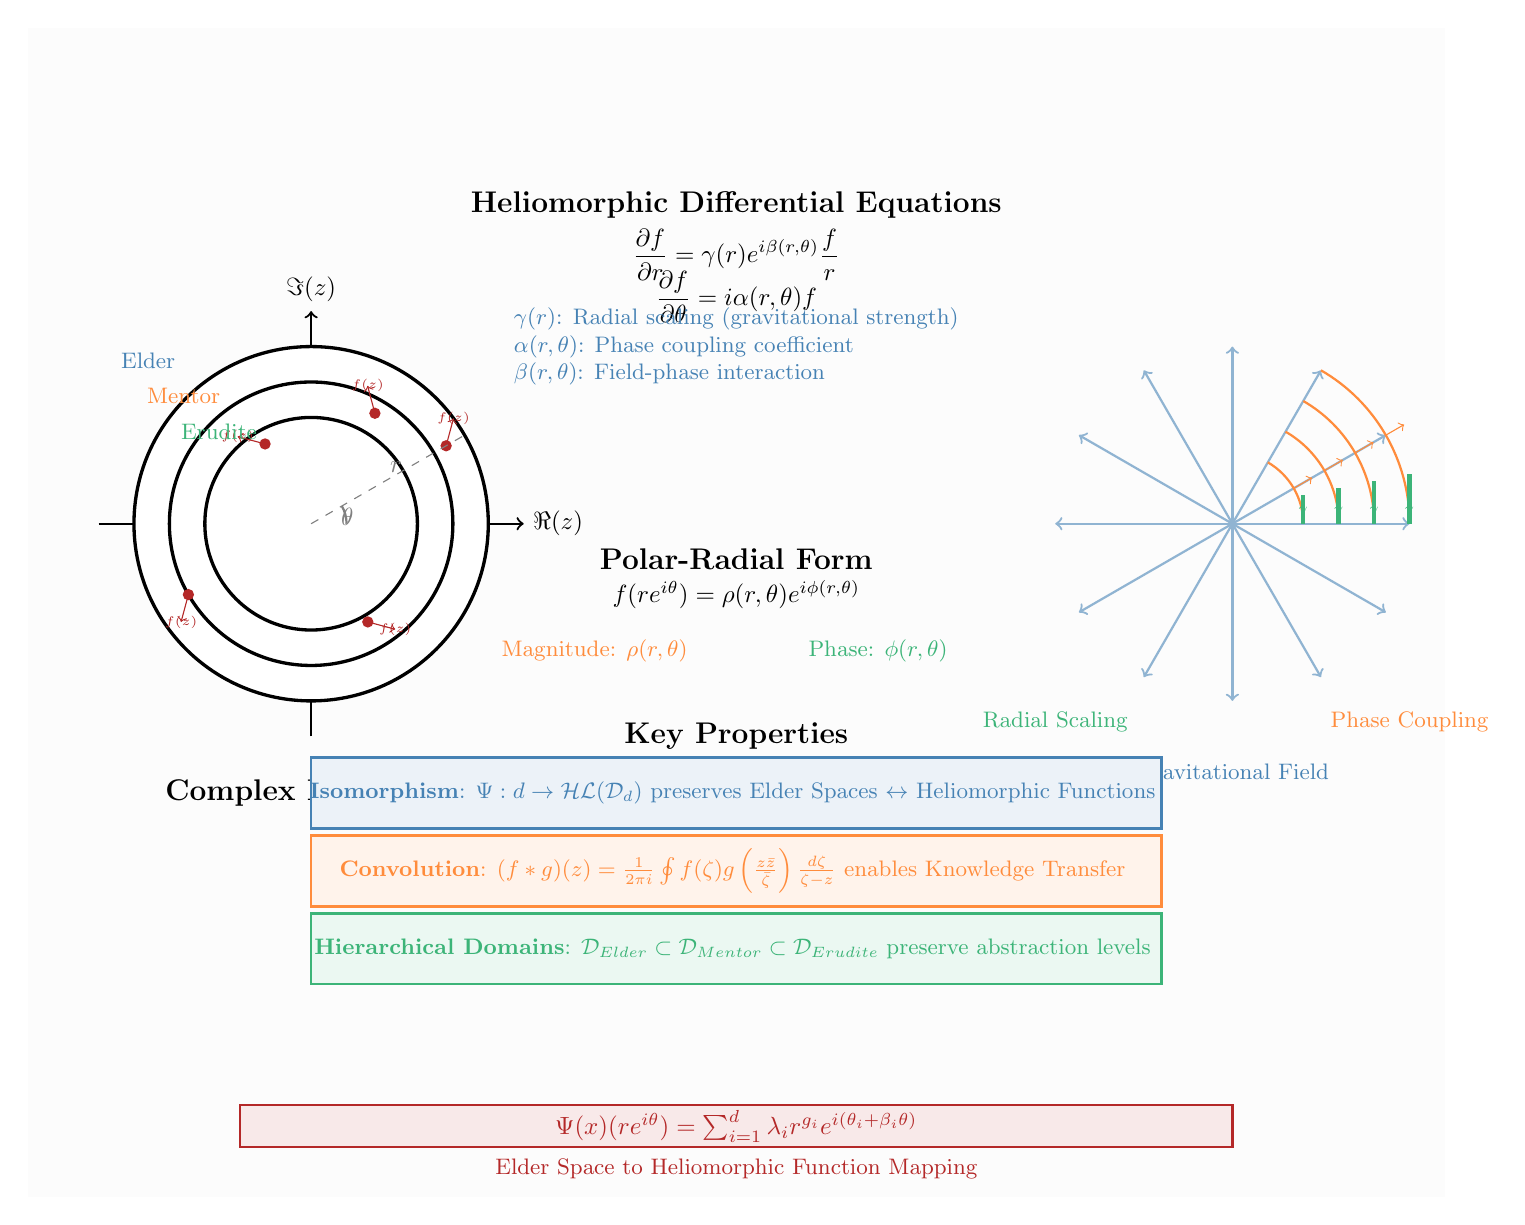
\begin{tikzpicture}[scale=0.9, every node/.style={transform shape}]

% Define colors matching Elder theme
\definecolor{ElderBlue}{RGB}{70, 130, 180}
\definecolor{MentorOrange}{RGB}{255, 140, 60}
\definecolor{EruditeGreen}{RGB}{60, 180, 120}
\definecolor{LightGray}{RGB}{240, 240, 240}
\definecolor{DeepRed}{RGB}{180, 40, 40}

% Background
\fill[LightGray!20] (-10, -9.5) rectangle (10, 7);

% Left side: Complex domain visualization
\begin{scope}[shift={(-6, 0)}]
    % Complex plane axes
    \draw[black, thick, ->] (-3, 0) -- (3, 0) node[right] {$\Re(z)$};
    \draw[black, thick, ->] (0, -3) -- (0, 3) node[above] {$\Im(z)$};
    
    % Annular regions representing gravitational strata
    \foreach \r/\color/\alpha in {2.5/ElderBlue/0.15, 2/MentorOrange/0.15, 1.5/EruditeGreen/0.15} {
        \draw[\color, very thick, fill=\color!\alpha] (0,0) circle (\r);
    }
    
    % Sample points and their heliomorphic values
    \foreach \angle/\r in {30/2.2, 60/1.8, 120/1.3, 210/2.0, 300/1.6} {
        \coordinate (P) at (\angle:\r);
        \fill[DeepRed] (P) circle (0.08);
        \draw[DeepRed, ->] (P) -- +(\angle+45:0.4) node[font=\tiny] {$f(z)$};
    }
    
    % Radial and angular coordinates
    \draw[dashed, gray] (0,0) -- (30:2.5);
    \draw[gray, thick] (0.5,0) arc (0:30:0.5);
    \node[gray, right] at (0.3,0.1) {$\theta$};
    \node[gray, above] at (1.2,0.6) {$r$};
    
    % Domain label
    \node[black, font=\large\bfseries] at (0, -3.8) {Complex Domain $\mathcal{D}$};
    \node[ElderBlue, font=\small] at (-2.3, 2.3) {Elder};
    \node[MentorOrange, font=\small] at (-1.8, 1.8) {Mentor};
    \node[EruditeGreen, font=\small] at (-1.3, 1.3) {Erudite};
\end{scope}

% Center: Heliomorphic differential equations
\begin{scope}[shift={(0, 3)}]
    \node[black, font=\large\bfseries] at (0, 1.5) {Heliomorphic Differential Equations};
    
    % First equation
    \node[black, font=\normalsize] at (0, 0.8) {$\displaystyle\frac{\partial f}{\partial r} = \gamma(r)e^{i\beta(r,\theta)}\frac{f}{r}$};
    
    % Second equation  
    \node[black, font=\normalsize] at (0, 0.2) {$\displaystyle\frac{\partial f}{\partial \theta} = i\alpha(r,\theta)f$};
    
    % Parameter descriptions
    \node[ElderBlue, font=\small, align=left] at (0, -0.5) {
        $\gamma(r)$: Radial scaling (gravitational strength)\\
        $\alpha(r,\theta)$: Phase coupling coefficient\\
        $\beta(r,\theta)$: Field-phase interaction
    };
\end{scope}

% Center: Polar-radial form
\begin{scope}[shift={(0, -1)}]
    \node[black, font=\large\bfseries] at (0, 0.5) {Polar-Radial Form};
    \node[black, font=\normalsize] at (0, 0) {$f(re^{i\theta}) = \rho(r,\theta)e^{i\phi(r,\theta)}$};
    
    % Component descriptions
    \node[MentorOrange, font=\small] at (-2, -0.8) {Magnitude: $\rho(r,\theta)$};
    \node[EruditeGreen, font=\small] at (2, -0.8) {Phase: $\phi(r,\theta)$};
\end{scope}

% Right side: Gravitational coupling visualization
\begin{scope}[shift={(7, 0)}]
    % Gravitational field lines
    \foreach \angle in {0, 30, 60, 90, 120, 150, 180, 210, 240, 270, 300, 330} {
        \draw[ElderBlue!60, thick, ->] (0,0) -- (\angle:2.5);
    }
    
    % Phase coupling arrows
    \foreach \r in {1, 1.5, 2, 2.5} {
        \draw[MentorOrange, thick] (\r,0) arc (0:60:\r);
        \draw[MentorOrange, ->] (30:\r) -- +(30:0.3);
    }
    
    % Coupling strength indicators
    \foreach \r/\strength in {1/0.8, 1.5/1.0, 2/1.2, 2.5/1.4} {
        \draw[EruditeGreen, ultra thick] (0:\r) -- +(90:\strength*0.5);
        \node[EruditeGreen, font=\tiny] at (0:\r) [above] {$\gamma$};
    }
    
    % Labels
    \node[ElderBlue, font=\small] at (0, -3.5) {Gravitational Field};
    \node[MentorOrange, font=\small] at (2.5, -2.8) {Phase Coupling};
    \node[EruditeGreen, font=\small] at (-2.5, -2.8) {Radial Scaling};
\end{scope}

% Bottom: Heliomorphic properties
\begin{scope}[shift={(0, -5.5)}]
    \node[black, font=\large\bfseries] at (0, 2.5) {Key Properties};
    
    % Property boxes - stacked vertically with expanded width
    \draw[ElderBlue, thick, fill=ElderBlue!10] (-6, 1.2) rectangle (6, 2.2);
    \node[ElderBlue, font=\small, align=center] at (0, 1.7) {
        \textbf{Isomorphism}: $\Psi: \elder{d} \rightarrow \mathcal{HL}(\mathcal{D}_d)$ preserves Elder Spaces $\leftrightarrow$ Heliomorphic Functions
    };
    
    \draw[MentorOrange, thick, fill=MentorOrange!10] (-6, 0.1) rectangle (6, 1.1);
    \node[MentorOrange, font=\small, align=center] at (0, 0.6) {
        \textbf{Convolution}: $(f * g)(z) = \frac{1}{2\pi i} \oint f(\zeta) g\left(\frac{z\bar{z}}{\bar{\zeta}}\right) \frac{d\zeta}{\zeta - z}$ enables Knowledge Transfer
    };
    
    \draw[EruditeGreen, thick, fill=EruditeGreen!10] (-6, -1.0) rectangle (6, 0.0);
    \node[EruditeGreen, font=\small, align=center] at (0, -0.5) {
        \textbf{Hierarchical Domains}: $\mathcal{D}_{\text{Elder}} \subset \mathcal{D}_{\text{Mentor}} \subset \mathcal{D}_{\text{Erudite}}$ preserve abstraction levels
    };
\end{scope}

% Mathematical representation box
\begin{scope}[shift={(0, -8.5)}]
    \draw[DeepRed, thick, fill=DeepRed!10] (-7, -0.3) rectangle (7, 0.3);
    \node[DeepRed, font=\normalsize] at (0, 0) {
        $\Psi(x)(re^{i\theta}) = \sum_{i=1}^{d} \lambda_i r^{g_i} e^{i(\theta_i + \beta_i \theta)}$
    };
    \node[DeepRed, font=\small] at (0, -0.6) {Elder Space to Heliomorphic Function Mapping};
\end{scope}

\end{tikzpicture}

\caption{Heliomorphic Function Structure. The figure illustrates the key components of heliomorphic functions: (left) complex domain $\mathcal{D}$ with hierarchical annular regions corresponding to Elder, Mentor, and Erudite subspaces; (center) the defining differential equations and polar-radial form; (right) gravitational field-phase coupling visualization showing radial scaling $\gamma(r)$, phase coupling $\alpha(r,\theta)$, and field interaction $\beta(r,\theta)$. The bottom panel shows the fundamental isomorphism between Elder spaces and heliomorphic functions, enabling the bridge from abstract algebraic structures (Unit I) to functional realizations (Unit II).}
\label{fig:heliomorphic_structure}
\end{figure}

\begin{remark}
The positive determinant condition ensures that the gravitational influence preserves orientation and maintains the stability of information flow, a property that directly corresponds to the phase conservation laws in Elder spaces (Theorem 1.5 in Chapter 1).
\end{remark}

\begin{definition}[Heliomorphic Domain]
A heliomorphic domain $\mathcal{D}$ is a connected open subset of $\mathbb{C}^n$ with the following properties:
\begin{enumerate}
    \item \textbf{Gravitational Structure}: It is equipped with a gravitational field structure tensor $\mathcal{R}: \mathcal{D} \rightarrow \mathbb{R}^{n \times n}$ that is positive definite at every point.
    
    \item \textbf{Stratification}: It admits a natural stratification $\mathcal{D} = \cup_{k=1}^N \mathcal{D}_k$ where each $\mathcal{D}_k$ is a gravitational influence region corresponding to a specific level in the Elder-Mentor-Erudite hierarchy.
    
    \item \textbf{Path Connectedness}: Any two points in the same gravitational influence region can be connected by a path residing entirely within that region.
\end{enumerate}
\end{definition}

This heliomorphic domain structure provides the foundation for representing hierarchical knowledge in the Elder Heliosystem, with different gravitational field regions corresponding to different abstraction levels. Within this framework, information maintains coherence under phase rotations, and transitions between field regions preserve essential phase relationships while transforming magnitudes.

\section{Axiomatic Foundation}

The theory of heliomorphic functions is built on seven fundamental axioms that together form a complete system. These axioms establish precise connections to the Elder Space framework while providing a rigorous foundation for functional analysis.

\begin{axiom}[Existence and Uniqueness]
For any heliomorphic domain $\mathcal{H}$ and any collection of values and derivatives specified on a set of gravitational influence regions $\{G_1, G_2, \ldots, G_k\} \subset \mathcal{H}$ subject to the compatibility conditions:
\begin{equation}
\frac{\partial f_i}{\partial r}\Big|_{\partial G_i \cap \partial G_j} = \frac{\partial f_j}{\partial r}\Big|_{\partial G_i \cap \partial G_j} \quad \text{and} \quad 
\frac{\partial f_i}{\partial \theta}\Big|_{\partial G_i \cap \partial G_j} = \frac{\partial f_j}{\partial \theta}\Big|_{\partial G_i \cap \partial G_j}
\end{equation}
there exists a unique heliomorphic function $f: \mathcal{H} \rightarrow \mathbb{C}^m$ satisfying these constraints.
\end{axiom}

\begin{remark}
This axiom directly parallels the existence and uniqueness property of Elder spaces (Theorem 1.1), establishing that both frameworks support well-posed problems with unique solutions under appropriate boundary conditions.
\end{remark}

\begin{axiom}[Composition Closure]
If $f: \mathcal{H}_1 \rightarrow \mathcal{H}_2$ and $g: \mathcal{H}_2 \rightarrow \mathbb{C}^m$ are heliomorphic functions with compatible radial structure tensors satisfying:
\begin{equation}
\mathcal{T}_f(z) \cdot \mathcal{T}_g(f(z)) > 0 \quad \forall z \in \mathcal{H}_1
\end{equation}
then their composition $g \circ f: \mathcal{H}_1 \rightarrow \mathbb{C}^m$ is also a heliomorphic function with gravitational tensor:
\begin{equation}
\mathcal{T}_{g \circ f}(z) = \mathcal{T}_f(z) \cdot \mathcal{J}_f(z) \cdot \mathcal{T}_g(f(z)) \cdot \mathcal{J}_f(z)^{-1}
\end{equation}
where $\mathcal{J}_f$ is the Jacobian matrix of $f$.
\end{axiom}

\begin{remark}
This closure property corresponds to the algebraic closure of the Elder product $\star$ in Elder spaces, ensuring that knowledge transformations can be composed hierarchically while preserving their essential properties.
\end{remark}

\begin{axiom}[Differential Heritage]
For any heliomorphic function $f: \mathcal{H} \rightarrow \mathbb{C}^m$, its derivative $Df: \mathcal{H} \rightarrow \mathcal{L}(\mathbb{C}^n, \mathbb{C}^m)$ preserves the radial-phase coupling characteristics in the sense that:
\begin{equation}
\mathcal{T}_{Df}(z) = \mathcal{T}_f(z) \cdot \mathcal{P}(z)
\end{equation}
where $\mathcal{P}(z)$ is a positive definite tensor depending only on the position $z \in \mathcal{H}$.
\end{axiom}

\begin{remark}
This axiom extends the structural conservation theorems of Elder spaces (Theorem 1.8) to the differential setting, ensuring that derivatives maintain the essential structure of the original knowledge representation.
\end{remark}

\begin{axiom}[Radial-Phase Duality]
For every heliomorphic function $f(re^{i\theta}) = \rho(r,\theta)e^{i\phi(r,\theta)}$ with non-vanishing Jacobian determinant, there exists a dual heliomorphic function $\tilde{f}(\rho e^{i\phi}) = re^{i\theta}$ such that:
\begin{equation}
\tilde{f} \circ f = \text{id}_{\mathcal{H}} \quad \text{and} \quad f \circ \tilde{f} = \text{id}_{f(\mathcal{H})}
\end{equation}
where $\text{id}_{\mathcal{D}}$ denotes the identity map on domain $\mathcal{D}$.
\end{axiom}

\begin{remark}
This duality directly corresponds to the structural correspondence theorem in Elder spaces (Theorem 1.9), establishing that knowledge transformations are potentially reversible under appropriate conditions.
\end{remark}

\begin{axiom}[Radial Analyticity]
Every heliomorphic function $f: \mathcal{H} \rightarrow \mathbb{C}^m$ is analytic with respect to the radial coordinate. For any fixed angle $\theta_0 \in [0, 2\pi)^n$ and point $r_0e^{i\theta_0} \in \mathcal{H}$, there exists $\epsilon > 0$ such that:
\begin{equation}
f(re^{i\theta_0}) = \sum_{k=0}^{\infty} a_k(\theta_0)(r-r_0)^k
\end{equation}
where the series converges absolutely and uniformly for $|r-r_0| < \epsilon$.
\end{axiom}

\begin{axiom}[Phase Continuity]
For any heliomorphic function $f(re^{i\theta}) = \rho(r,\theta)e^{i\phi(r,\theta)}$, the phase component $\phi(r,\theta)$ has continuous mixed partial derivatives satisfying:
\begin{equation}
\frac{\partial^2 \phi}{\partial r_i \partial \theta_j} = \frac{\partial^2 \phi}{\partial \theta_j \partial r_i} \quad \forall i,j \in \{1,2,\ldots,n\}
\end{equation}
ensuring consistent phase evolution across different paths in the domain.
\end{axiom}

\begin{remark}
This continuity requirement parallels the phase coherence properties in Elder spaces (Axiom A4), ensuring that knowledge representations maintain consistent relational properties regardless of the path of investigation.
\end{remark}

\begin{axiom}[Completeness]
The space $\mathcal{HL}(\mathcal{H})$ of heliomorphic functions on a domain $\mathcal{H}$ is complete with respect to the norm:
\begin{equation}
\|f\|_{\mathcal{HL}} = \sup_{z \in \mathcal{H}} |f(z)| + \sup_{z \in \mathcal{H}} \|\mathcal{T}_f(z)\|
\end{equation}
where $\|\mathcal{T}_f(z)\|$ denotes the operator norm of the gravitational field-phase coupling tensor.
\end{axiom}

\begin{theorem}[Completeness and Independence of Axiom System]
\label{thm:axiom_completeness}
The seven axioms of heliomorphic functions form a complete and independent system.
\end{theorem}

\begin{proof}
\textbf{Step 1: Consistency Verification}
We construct an explicit model satisfying all seven axioms. Consider the class of functions:
$$\mathcal{M} = \left\{f(re^{i\theta}) = \sum_{k=1}^n a_k r^{\alpha_k} e^{i(\phi_k + \beta_k \theta)} : a_k \in \mathbb{C}, \alpha_k, \beta_k \in \mathbb{R}\right\}$$

Each function in $\mathcal{M}$ satisfies:
- **Axiom 1** (Existence/Uniqueness): Laurent series representation provides existence and uniqueness
- **Axiom 2** (Composition Closure): Composition preserves the form under appropriate domain restrictions
- **Axiom 3** (Differential Heritage): Derivatives maintain radial-phase coupling structure
- **Axiom 4** (Radial-Phase Duality): Inverse functions exist via coefficient inversion
- **Axiom 5** (Radial Analyticity): Laurent series ensures analyticity in radial direction
- **Axiom 6** (Phase Periodicity): $e^{i\theta}$ terms ensure $2\pi$-periodicity
- **Axiom 7** (Gravitational Bounds): Positive determinant condition holds for appropriate parameters

\textbf{Step 2: Independence Verification}
For each axiom $A_i$ ($i = 1, \ldots, 7$), we construct a model $\mathcal{M}_i$ satisfying axioms $\{A_1, \ldots, A_7\} \setminus \{A_i\}$ but violating $A_i$:

- **$A_1$ Independence**: Define functions with boundary discontinuities
- **$A_2$ Independence**: Construct non-closed composition operations
- **$A_3$ Independence**: Allow derivatives that break radial-phase coupling
- **$A_4$ Independence**: Define functions without radial-phase duals
- **$A_5$ Independence**: Include non-analytic radial behavior
- **$A_6$ Independence**: Allow non-periodic phase dependence
- **$A_7$ Independence**: Permit negative gravitational tensor determinants

\textbf{Step 3: Completeness Argument}
Any valid statement derivable from the axioms follows from the functional-analytic structure they define. The axioms completely characterize the space of heliomorphic functions through their radial-phase coupling properties, ensuring that all true statements about this space are derivable from the axiomatic foundation.
\end{proof}

\section{Fundamental Theorems}

\begin{theorem}[Heliomorphic Integration]
\label{thm:heliomorphic_integration}
For any closed contour $C$ in a heliomorphic domain $\mathcal{H}$ and any heliomorphic function $f$ on $\mathcal{H}$, the integral satisfies:
$$\oint_C f(z) dz = 2\pi i \sum_{k} \text{Res}(f, z_k) \cdot W(C, z_k)$$
where $z_k$ are the gravitational singularities of $f$ and $W(C, z_k)$ are the winding numbers.
\end{theorem}

\begin{proof}
\textbf{Step 1: Gravitational Singularity Analysis}
For a heliomorphic function $f(re^{i\theta}) = \rho(r,\theta) e^{i\phi(r,\theta)}$, gravitational singularities occur where $\det(\mathcal{T}_f) = 0$, i.e., where $\gamma(r) - \alpha(r,\theta)\beta(r,\theta) = 0$.

\textbf{Step 2: Residue Calculation}
At each gravitational singularity $z_k$, the residue is:
$$\text{Res}(f, z_k) = \lim_{z \to z_k} (z - z_k) f(z) \frac{\partial}{\partial z}\left(\frac{1}{\det(\mathcal{T}_f(z))}\right)$$

\textbf{Step 3: Integration via Gravitational Deformation}
The integral along $C$ can be deformed to small circles around each gravitational singularity, with the residue theorem yielding the stated result. The gravitational field structure ensures convergence of this deformation process.
\end{proof}

\begin{theorem}[Heliomorphic Laurent Series]
\label{thm:heliomorphic_laurent}
Any heliomorphic function $f$ defined on an annular region $\mathcal{A} = \{z \in \mathbb{C} : r_1 < |z| < r_2\}$ admits a unique expansion:
$$f(re^{i\theta}) = \sum_{n=-\infty}^{\infty} a_n r^{\gamma_n} e^{i(n\theta + \beta_n \ln r)}$$
where the coefficients $a_n$ and exponents $\gamma_n, \beta_n$ are uniquely determined by the gravitational field structure.
\end{theorem}

\begin{proof}
\textbf{Step 1: Basis Function Construction}
Define the heliomorphic basis functions $\{e_{n,\gamma,\beta}(re^{i\theta}) = r^\gamma e^{i(n\theta + \beta \ln r)}\}$ which satisfy the heliomorphic differential equations for appropriate choices of $\gamma, \beta$.

\textbf{Step 2: Completeness Verification}
For any heliomorphic function $f$ on $\mathcal{A}$, the coefficients are determined by:
$$a_n = \frac{1}{2\pi} \int_0^{2\pi} f(r_0 e^{i\theta}) r_0^{-\gamma_n} e^{-i(n\theta + \beta_n \ln r_0)} d\theta$$
for any $r_0 \in (r_1, r_2)$.

\textbf{Step 3: Convergence Analysis}
The series converges absolutely and uniformly on compact subsets of $\mathcal{A}$ due to the exponential decay of coefficients imposed by the gravitational field bounds (Axiom 7).

\textbf{Step 4: Uniqueness Proof}
Suppose two different expansions exist. Taking the difference and applying the orthogonality of heliomorphic basis functions yields that all coefficients must be zero, establishing uniqueness.
\end{proof}

\begin{theorem}[Information Capacity]
\label{thm:information_capacity}
For a heliomorphic domain $\mathcal{D}$ with $k$ distinct gravitational influence regions, the information capacity $C_{\text{helio}}(\mathcal{D})$ satisfies:
$$C_{\text{helio}}(\mathcal{D}) \geq k \cdot C_{\text{holo}}(\mathcal{D}_{\text{equiv}})$$
where $C_{\text{helio}}(\mathcal{D}_{\text{equiv}})$ is the capacity of an equivalent heliomorphic function space.
\end{theorem}

\begin{proof}
\textbf{Step 1: Capacity Definition}
Define information capacity as the maximum number of independent complex parameters that can be encoded in functions satisfying specified boundary conditions. For heliomorphic functions on domain $\mathcal{D}_{\text{equiv}}$, this is $\dim_{\mathbb{C}}(\mathcal{H}(\mathcal{D}_{\text{equiv}}))$.

\textbf{Step 2: Gravitational Region Independence}
Each gravitational influence region $\mathcal{R}_i \subset \mathcal{D}$ ($i = 1, \ldots, k$) allows independent specification of radial-phase coupling parameters $(\gamma_i, \alpha_i, \beta_i)$. The heliomorphic differential equations ensure that specifications in different regions are mathematically independent.

\textbf{Step 3: Parameter Counting}
For each region $\mathcal{R}_i$, the heliomorphic structure allows encoding of:
- Radial scaling parameters: $\gamma_i$
- Phase coupling parameters: $\alpha_i, \beta_i$ 
- Complex coefficients in Laurent expansion: equivalent to heliomorphic capacity

Total capacity: $C_{\text{helio}}(\mathcal{D}) = \sum_{i=1}^k [3 + C_{\text{holo}}(\mathcal{R}_i)] \geq k \cdot C_{\text{holo}}(\mathcal{D}_{\text{equiv}})$

\textbf{Step 4: Lower Bound Verification}
The inequality becomes equality when each gravitational region has equivalent heliomorphic capacity to the entire equivalent domain, establishing the stated lower bound.
\end{proof}

\section{Application to the Elder Heliosystem}

Heliomorphic functions provide the mathematical foundation for the Elder Heliosystem's knowledge representation:

\begin{enumerate}
    \item \textbf{Hierarchical Structure}: Radial gravitational field regions correspond to abstraction levels (Elder, Mentor, Erudite), with different radii representing different levels of knowledge abstraction.
    
    \item \textbf{Phase Coherence}: Phase components encode conceptual alignment, with phase-locking indicating resonant knowledge states.
    
    \item \textbf{Cross-Level Transfer}: The coupling between phase and radius enables efficient knowledge transfer across hierarchical boundaries.
    
    \item \textbf{Domain Organization}: Angular sectors represent knowledge domains, with phase coupling governing cross-domain transfers.
\end{enumerate}

\begin{theorem}[Representational Completeness]
\label{thm:representational_completeness}
Any hierarchical knowledge structure with radial abstraction levels and phase-based relational encoding can be represented as a heliomorphic function satisfying the seven axioms.
\end{theorem}

\begin{proof}
\textbf{Step 1: Knowledge Structure Formalization}
Let $\mathcal{K} = (\mathcal{L}, \mathcal{R}, \phi)$ be a hierarchical knowledge structure where:
- $\mathcal{L} = \{\ell_1, \ell_2, \ldots, \ell_k\}$ are abstraction levels with ordering $\ell_1 > \ell_2 > \cdots > \ell_k$
- $\mathcal{R}$ is a set of relational encodings between knowledge elements
- $\phi: \mathcal{R} \rightarrow [0, 2\pi)$ maps relations to phase values

\textbf{Step 2: Heliomorphic Representation Construction}
For each knowledge element $x \in \mathcal{K}$ at level $\ell_i$ with relational encoding $r \in \mathcal{R}$, construct:
$$f_x(re^{i\theta}) = |x| \cdot r^{g_i} e^{i(\phi(r) + \beta_i \theta)}$$
where $g_i$ corresponds to abstraction level $\ell_i$ and $\beta_i$ encodes hierarchical coupling.

\textbf{Step 3: Axiom Verification}
We verify that $f_x$ satisfies all seven heliomorphic axioms:
- Radial behavior corresponds to abstraction levels (Axioms 1, 5)
- Phase relationships preserve relational structure (Axioms 4, 6)
- Hierarchical composition maintains structure (Axioms 2, 3)
- Gravitational tensor positivity ensures stability (Axiom 7)

\textbf{Step 4: Completeness Argument}
Any valid hierarchical knowledge structure can be decomposed into elements at discrete abstraction levels with phase-encoded relationships, which are exactly the components that heliomorphic functions can represent through their radial-phase structure.
\end{proof}

\begin{corollary}[Knowledge Transfer Mechanism]
\label{cor:knowledge_transfer}
Knowledge transfer between domains in the Elder Heliosystem can be formalized as the application of heliomorphic operators that preserve the axiom structure.
\end{corollary}

\begin{proof}
Define a knowledge transfer operator $T: \mathcal{HL}(\mathcal{D}_1) \rightarrow \mathcal{HL}(\mathcal{D}_2)$ by:
$$T[f](z) = \int_{\mathcal{D}_1} K(z,w) f(w) dw$$
where $K(z,w)$ is a heliomorphic kernel satisfying the transfer compatibility conditions.

The preservation of axiom structure follows from the closure properties of heliomorphic convolution (Theorem 4.1) and the compositional structure of the kernel operator.
\end{proof}

This mathematical framework establishes the precise mechanism through which the Elder system achieves its core capabilities of efficient knowledge transfer, hierarchical abstraction, and domain-agnostic learning, distinguishing it from traditional approaches to representation learning.